\section{Análisis Espacial de Estructuras de Datos}
\subsection{Propuestas}
Analizamos las distintas alternativas para almacenar la matriz esparsa en términos de eficiencia espacial, comparando en qué casos una alternativa es mejor que otra. Tenemos 4 posibles estructuras de datos para almacenar la matriz. Las opciones propuestas son: \\

\begin{itemize}
	\item \textbf{Vector}: Consiste en almacenar la matriz en un único vector del tamaño de la matriz, almacenando todos los valores de la misma incluyendo los valores nulos.  
	\item \textbf{Dictionary Of Keys (DOK)}: Consiste en almacenar los valores de la matriz que no son nulos en un diccionario, donde las \textit{keys} son la dupla fila y columna, y el \textit{value} es el valor en esa posición. Si una posición no se encuentra en el diccionario, significa que el valor en esa posición es cero.
	\item \textbf{Compressed Sparse Row (CSR)}: Consiste en utilizar 3 \textit{arrays}, uno para guardar todos los valores distintos de cero, otro para guardar la columna donde se encuentran los elementos anteriores, y por último uno donde se almacenan los índices de el primer elemento distinto de cero para cada fila.
	\item \textbf{Compressed Sparse Column (CSC)}: Es igual al CSR, sólo que en lugar de almacenar por filas, se almacena por columnas. El primer \textit{array} guarda los mismos valores pero por columnas, el segundo indica la fila de cada elemento y el último indica el primer elemento distinto de cero de cada columna. La cantidad de memoria que utiliza es exactamente la misma que CSR, dado que los dos primeros $arrays$ tienen igual tamaño (la cantidad de elementos no nulos), y al ser la matriz cuadrada, la cantidad de filas es igual a la de las columnas, coincidiendo así el tamaño del tercer $array$.
\end{itemize}

Para el análisis temporal, optamos por utilizar los valores reales de tamaño que se utiliza en C++, dado que realizando un análsis teórico se llegan a conclusiones que no se corresponden con la implemetación. Un ejemplo sería pensar que una lista de $n$ elementos de tamaño $size\_of\_element$ ocupa un tamaño de $n*size\_of\_element$, cuando en realidad, dependiendo de la implementación, es necesario también tener en cuenta el costo espacial de los punteros para la lista. Si esto no es tenido en cuenta, se podría optar por una estructura de datos que en realidad ocupe más espacio del pensado comparado contra otras alternativas. \\
Para los indices utilizamos el tipo $int$, cuyo tamaño es de 4 bytes, mientras que para los valores almacenados en la matriz utilizamos el tipo $double$ cuyo tamaño es 8 bytes. Para los indices se podría utilizar como alternativa \textit{unsigned int}, que también tienen un tamaño de 4 bytes.\\
Definimos \textbf{NNZ} (NonZero) como la cantidad de valores no nulos de la matriz y $n$ la cantidad de filas (coincidente con las columnas dado que es cuadrada). \\

\subsection{Análisis:}
Para todos los casos, se midió la cantidad de memoria reservada utilizando \textit{valgrind}. Utilizamos para cada caso un pequeño programa que genera una instancia para cada estructura, primero vacía, y luego agregando elementos. De este modo, pudimos observar cuanta memoria utiliza cada estructura por separado. Los resultados del uso de memoria fueron:\\
%http://netlib.org/linalg/html_templates/node91.html

\begin{itemize}
	\item \textbf{Vector}: $n^2 * 8\ bytes$
	\item \textbf{Dictionary Of Keys (DOK)}: $NNZ * 48\ bytes$
	\item \textbf{Compressed Sparse Row (CSR)}: $8*NNZ + 4*NNZ + 4 (n+1)\ bytes$
\end{itemize}

Fue útil tener en cuenta la cantidad de memoria real, principalmente para constatar que tanto Vector como CSR usaran la cantidad teórica estimada, además de saber que DOK utiliza una cantidad mayor a la pensada. Esto se debe a que DOK está implementado sobre el tipo $map$ de C++, que es un Black-Red Tree. Cada elemento cuesta 48 bytes, más que un double ($value$) y dos enteros ($key$), que serían 16 bytes.  \\

Existen casos para los cuales, cada una de las alternativas anteriores es mejor que el resto. Para ejemplificarlo, supongamos que se tiene una matriz con tamaño $n=100$. Graficamos la cantidad de memoria requerida por cada estructura, variando la cantidad de valores distintos de cero: \\

\begin{wrapfigure}{r}{0.6\textwidth}
  \vspace{-20pt}
  \begin{center}
    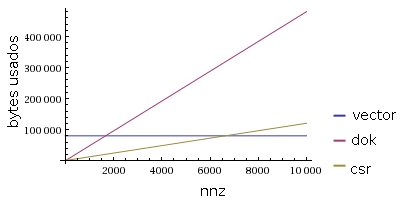
\includegraphics[scale= 0.6]{imagenes/n100espacio.png}
  \end{center}
  \vspace{-20pt}
   \caption[Caption espacio n 100]{Memoria utilizada en una matriz de tamaño 100x100, variando la cantidad de valores no nulos}
  \vspace{-10pt}
  \label{fig:img1}
\end{wrapfigure}

Cabe destacar que, a pesar de no notarse en el gráfico, el Dictionary Of Keys utiliza menos memoria que Compressed Sparse Row para cuando hay menos de 12 valores distintos de cero. A partir de $12 \leq nnz$, Dictionary Of Keys utiliza más memoria.
